
%%%%%%%%%%%%%%%%%%%%%%% file typeinst.tex %%%%%%%%%%%%%%%%%%%%%%%%%
%
% This is the LaTeX source for the instructions to authors using
% the LaTeX document class 'llncs.cls' for contributions to
% the Lecture Notes in Computer Sciences series.
% http://www.springer.com/lncs       Springer Heidelberg 2006/05/04
%
% It may be used as a template for your own input - copy it
% to a new file with a new name and use it as the basis
% for your article.
%
% NB: the document class 'llncs' has its own and detailed documentation, see
% ftp://ftp.springer.de/data/pubftp/pub/tex/latex/llncs/latex2e/llncsdoc.pdf
%
%%%%%%%%%%%%%%%%%%%%%%%%%%%%%%%%%%%%%%%%%%%%%%%%%%%%%%%%%%%%%%%%%%%


\documentclass[runningheads,a4paper]{llncs}

\usepackage{amssymb}
\setcounter{tocdepth}{3}
\usepackage{graphicx}
\usepackage{epstopdf}

\usepackage{url}
\urldef{\mailsa}\path|{wilhelmm, jgartner, yimingf, shamaei, mutas}@kth.se|
\newcommand{\keywords}[1]{\par\addvspace\baselineskip
\noindent\keywordname\enspace\ignorespaces#1}

\begin{document}

\mainmatter  % start of an individual contribution

% first the title is needed
\title{Clustering People in Social Network Based on Graph Databases}

% a short form should be given in case it is too long for the running head
\titlerunning{Lecture Notes in Computer Science: Authors' Instructions}

% the name(s) of the author(s) follow(s) next
%
% NB: Chinese authors should write their first names(s) in front of
% their surnames. This ensures that the names appear correctly in
% the running heads and the author index.
%
\author{Wilhelm Magnusson\and Joel G\"artner\and Yiming Fan\and\\ Sepideh Shamaei\and Mahmut U\u{g}ur Ta\u{s}}
%
\authorrunning{Clustering People in Social Network Based on Graph Databases}
% (feature abused for this document to repeat the title also on left hand pages)

% the affiliations are given next; don't give your e-mail address
% unless you accept that it will be published
\institute{KTH Royal Institute of Technology,\\
SE-10044, Stockholm, Sweden\\
\mailsa}

%
% NB: a more complex sample for affiliations and the mapping to the
% corresponding authors can be found in the file "llncs.dem"
% (search for the string "\mainmatter" where a contribution starts).
% "llncs.dem" accompanies the document class "llncs.cls".
%

\toctitle{Lecture Notes in Computer Science}
\tocauthor{Authors' Instructions}
\maketitle

\begin{abstract}
We have found efficient ways of structuring and searching through clusters of Facebook event data in order to find connections between people with similar interests. This was done by fetching data through Facebook��s public API and testing and optimising the data structure for the algorithms described in the paper GraphSystems-tutorial�. The output has DBMS form that can find people based on how similar their interests are using a graph database and a small sample size of peoples event data from Facebook.
\end{abstract}

\section{Introduction}
The everyday use of social network has grown explosively. Therefore, it is an interesting mission for data analysers to retrieve useful facts from the massive data. Traditional RDBMS are relatively ad-hoc and computation consuming, and they have been replaced by light-weight and efficient \texttt{NoSQL} database systems. One widely adapted database system, the graph database, could represent and store massive data with the structure of nodes and edges. This hierarchical structure allows retrievals which are relatively rapid, comparing to conventional database systems. Its performance surpasses most conventional database systems when handling with graph-like queries. \cite{graph}

Clustering users is an important task in social network data mining. Users may be recognised with respect to their ages, locations, occupations, marital status, and/or interests. Some machine learning methods, for example, Self-Organizing Maps (SOM) are proved to efficiently cluster people at various scales. Our project group, on the other hand, has implemented some clustering method based on graph queries. It utilises the advantages of graph data structure among various users, and has a relatively fair scoring scale. We also implemented a comparing group with the form of conventional RDBMS, in order to compare their performance.

\section{Method \& Implementation}
\subsection*{Facebook data}
First of all, data was required to be fetched with the Facebook API. This was done with the help of a 
\texttt{python} module called \texttt{facepy} which allowed calls to the API from within \texttt{python}. In order to get interesting data from this, the
solution was to search for events located within a 20-km radius from a point in Stockholm. The 
persons used in the experiment was then the persons which attended these events and the only
events used were the ones found in this way.

As a result, we have fetched $2000$ events, $73981$ persons
and in total $140713$ attending relationships in the databases. This means that
for the fetched data each person was in average in about two of the events which
were fetched.

\subsection*{Graph database}
The graph database used was the community edition of \texttt{Neo4j}. In order to make queries and
make graphs in \texttt{Neo4j} the \texttt{cypher} language is used. This was used to load the data
and create a graph which had two types of nodes, namely \textit{events} and
\textit{persons}. A relation from persons to events called \textit{Attending} was also created for
each persons to all events they attended. With this graph in place it was, once 
getting familiar with the language, relatively easy to do the desired query
for a person with a given \textit{id}.
For the person with \textit{id} $123$ this was done with the command
\begin{verbatim}
MATCH (p:Person {id : 123})-->(e:Event),(e)<--(q:Person) 
RETURN q,Count(q) AS nr ORDER BY nr DESC;
\end{verbatim}
which simply finds all persons which the person has been on events with and orders
them by how many events they have attended together.

\subsection*{SQL}
An equivalent query was implemented in \texttt{sql} in order to get a comparison with a traditional RDBMS.
In \texttt{sql} the data was loaded into three tables, \textit{persons}, \textit{events} and \textit{attending} where 
the \textit{attending} table was a many-to-many relation between \textit{persons} and \textit{events}.
In order to construct the query it was simply to do a join between two
copies of the \textit{attending} table over equal event \textit{id}s. By selecting all
entries in this joined table for which one of the copies of \textit{attending} has a specific user \textit{id} we will all persons who have attended events
with that persons. By simply counting the number of occurrences of 
a specific person this will give the same result as from the graph 
database.

% illustrate the method (graph db and traditional rdbms, if necessary)
% show some lines of code if necessary
\section{Results}
\subsection*{Query results}
Figure \ref{fig:graph} shows an example for how the graph looked in the web-interface.
In this specific graph it shows all events the person in red have attended as well
as all persons who attended these events, together with all the relations. Some comparisons were however performed to 
ensure that the data from the different queries was the same.
\begin{figure}
    \centering
    \def\svgwidth{\columnwidth}
    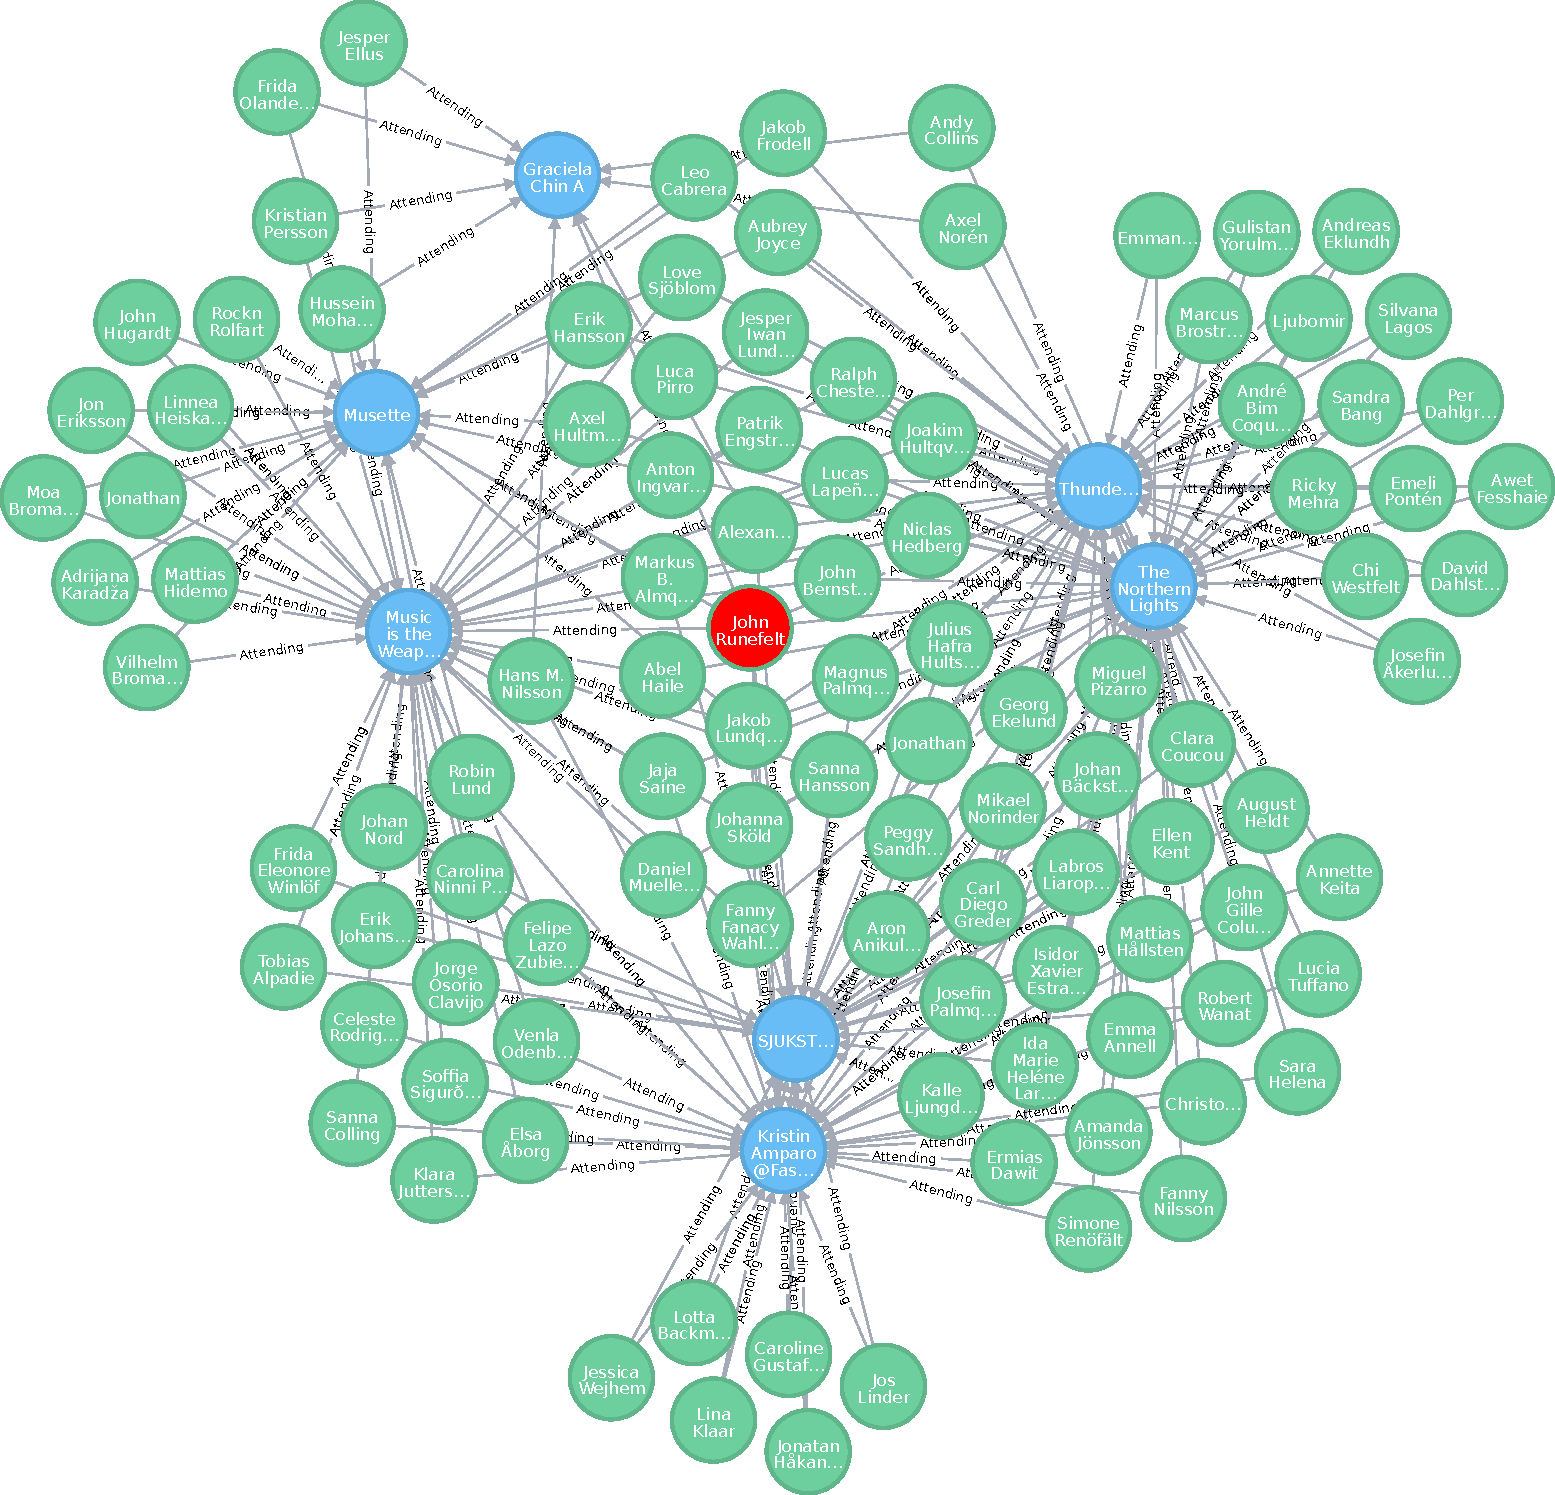
\includegraphics[width=10cm]{image.pdf}
    \caption{An example of the resulting graph}
    \label{fig:graph}
\end{figure}
\subsection*{Performance}
Some tests were performed on the performance of the implementations in the
different database structures. Initial testing was performed using the
\texttt{Neo4j} web-interface and direct commands to an \texttt{sqlite} database. This gave the 
result that the graph database was quite slower than the standard
relational database. A possible factor in this was however probably some added
overhead in the web-interface and the time spent was still mostly used for 
the output of the results. In order to get better results a Java-program was 
developed which used \texttt{sqlite} and \texttt{Neo4j Java} API:s. This program could then run
the queries and time them in different ways.

Trying this it however became clear that there was no obvious way to 
objectively measure the time for running the query. One reason for 
this was that the queries were constructed so that they picked out $N$ persons
and found the persons they had been on events with. The problem was then that
the $N$ persons which \texttt{Neo4j} picked and the $N$ persons which \texttt{sql} picked were
not the same. In order to still get interesting queries several queries were
performed. We first did the ``native'' query which resulted in the different
databases getting different results as they selected different persons initially.
For the rest of the queries we instead first selected the users from \texttt{sql} and
saved them in a list in Java. This list was used mainly for a loop where each
person selected was iterated over and then sent to a query for the respective 
languages. It was also used directly with the \texttt{Neo4j} API as it was possible
to supply iterable \texttt{Java} objects to it which would result in a collection
which was usable in the \texttt{cypher} language. This was used to directly insert the
list of selected users into the \texttt{cypher} query. The run-times for these queries
for different values of $N$ is shown in table \ref{tab:times}. Worth noting
is that in all runs of the native version the \texttt{Neo4j} query resulted in more 
result lines which is shown in table \ref{tab:nr}. The running times are
rounded to the nearest millisecond but in truth the running time varied by 
a lot more than that so the numbers are only indicators of behaviour 
and not average run times over multiple attempts.
\begin{table}
    \centering
    \begin{tabular}{|c|c|c|c|c|}
        \hline
        N & 1 & 10 & 100 & 300 \\
        \hline
        \texttt{Neo4j} native & 1416 & 585 & 900 & 2685 \\
        \hline
        SQL native   & 213 & 482 & 549 & 859 \\
        \hline
        \texttt{Neo4j} loop   & 76 & 1644 & 4535 & 5829 \\
        \hline
        SQL loop     & 207 & 1885 & 18510 & 54713 \\
        \hline
        \texttt{Neo4j} Java collection & 1143 & 3243 & 22937 & 65709 \\
        \hline
    \end{tabular}
    \caption{Running times in ms for different $N$}
    \label{tab:times}
\end{table}
\begin{table}
    \centering
    \begin{tabular}{|c|c|c|c|c|}
        \hline
        N & 1 & 10 & 100 & 300 \\
        \hline
        \texttt{Neo4j} & 7232 & 30266 & 52115 & 281550 \\
        \hline
        SQL & 170 & 9102 & 71090 & 194833 \\
        \hline
    \end{tabular}
\caption{Number result lines for different $N$ for native approach}
    \label{tab:nr}
\end{table}

\section{Discussion}
Surprisingly, the results above slightly object to what \texttt{Neo4j}'s official website says:
\begin{table}
\centering
\begin{tabular}{c|c|c}
depth & \texttt{Neo4j} & RDBMS\\
\hline
1 & .... & .....\\
2 & 0.01& 0.016\\
3 & 0.168 & 30.267\\
4 & 1.359 & 1543.505\\
5 & 2.132 & unfinished
\end{tabular}
\caption{Performance difference (in seconds) on multiple join query test. Claims from the book \textit{\texttt{Neo4j} in Action}, chapter 1, table 2-1}
\label{tab:pc}
\end{table}\\
However, we are not the only few who are curious about the difference between the claim and the result. J\"org Baach \cite{url} has doubted, that to achieve the dominating performance of \texttt{Neo4j} over \texttt{mysql}, one must set his/her operating environment carefully. However, environment issue could not confine a web developer in performance that much, or it disobeys the principle of reusability. Consider a project whose speed is stuck just by changing another computer. Maybe \texttt{Neo4j} is quicker under some certain test cases, but that is not the real use-case.

So could we end up discussing and say, ``gee, graph database sucks, let's roll back to traditional database''? The answer is far from true. In Jouili and Vansteenberghe's research \cite{graph} we found out, that \texttt{Neo4j} shares the similar performance with other graph database systems, such as \texttt{DEX} and \texttt{Titan}, in read-only workload, but would have a sharp performance degrade on read-write workload. Perhaps \texttt{Neo4j} is old-fashioned, high environment-demanding and slow, but we could have plenty of alternatives.

\section{Summary}
We presented Facebook friends clustering, using graph database system and traditional relational database. However, this real-life test case did not make a testimony that graph database is somehow great. This may due to incorrect computer configuration or bad computer environment, but considering the not-so-different personal-use computer capability, we're afraid that the very thing left to blame could be the improper choice of the graph database system. In the future we could do more test on different graph database systems to test their performance.\\

\begin{thebibliography}{4}

\bibitem{book} Vukotic, A., Partner, J., Watt, N., Abedrabbo, T., Fox, D.: \texttt{Neo4j} in Action. Manning, Greenwich (2014)

\bibitem{url} Baach, J.: neo4j performance compared to mysql, \url{http://baach.de/Members/jhb/neo4j-performance-compared-to-mysql}

\bibitem{graph} Jouili, S., Vansteenberghe, V.: An empirical comparison of graph databases. In: Social Computing (SocialCom), 2013 International Conference on, pp. 708--715. IEEE Press, Alexandria (2013)
\end{thebibliography}

\end{document}
